\documentclass[../Bitcoin Blink.tex]{subfiles}
\graphicspath{{\subfix{../assets/images/}}}
\begin{document}

\section{Bitcoin (Blink)} 
\subsection{Election}
Block size denotes the amount of data that can be propagated across every node on the Bitcoin network hence, its success rate is directly dependent on the bandwidth each node allocates for confirmed block transmission. Block size is not limited and is fixed in every new block, which denotes that every validator of the block can send and receive the data size. Variable block size helps to scale the network by increasing transactions per block when the nodes upgrade and announce their bandwidth. A ZK-SNARK-based proof takes a node’s bandwidth as a public input signal, which is compared to the threshold range of the desired bandwidth of the network. To prevent tampering, the node will commit a salt, which is a large random number that will be added to the bandwidth to generate the $xyz$ hash which will be verified in the proof. Thus, the proof will attest its bandwidth output to the UTXO’s script and get validated. 
\begin{figure}[h]
\begin{center}
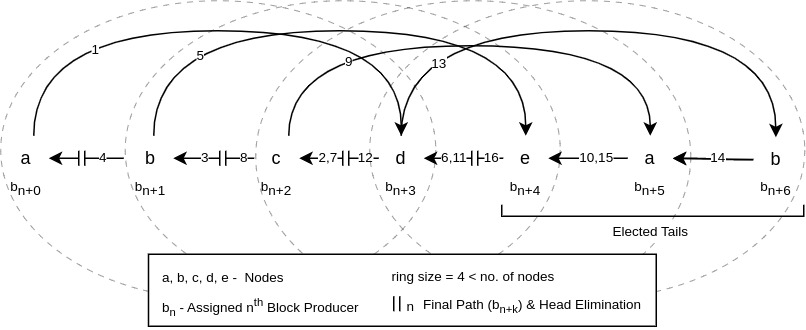
\includegraphics[width=11cm]{ring}
\caption{Ring Validation}
\label{ring}
\end{center}
\end{figure}
The network in consensus can forbid low bandwidth nodes from participating in the election to produce blocks. Bandwidth requirements are increased for nodes to get elected for next block production can assure the capacity to hold more transactions to scale further. Elections will be conducted based on nodes bandwidth and each node's honesty weight. Nodes identities are masked by their public keys encouraging privacy. For each block, the elected node will produce, and set of nodes will validate and attach to the longest chain \cite{nakamoto2008bitcoin} . This set of nodes are finite and unique for every block and are called as a ``ring validators" (see Fig.\ref{ring}). After each block's confirmation, the head of the ring is eliminated and a tail is elected which can be validated by nodes during propagation. The ring head after receiving the confirmed block will acquire bandwidth to gossip it's block over to other full or SPV nodes to secure it's rewards. The tail election's random seed is taken from concatenating Merkle Chain root and VDF Proof \cite{yakovenko2018solana} of the recent head's confirmed block. Thus, the election is conducted for every block where a tail node is assigned.

\end{document}
